\begin{figure}[ht!]
  \centering
\begin{subfigure}{.5\linewidth}
\centering
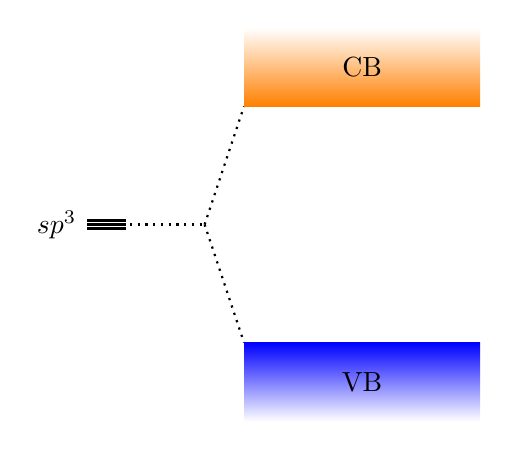
\begin{tikzpicture}

  \atom[name=C, color=orange, pos={(-2,0)},scale=0.5]{
    gray/45/45/0,
    gray/315/315/0,
    gray/225/225/0,
    gray/135/135/0}

  \draw[thick,-] (-1.5,-4) -- (-2.0,-4) node[anchor=east]{$sp^3$};
  \draw[thick,-] (-1.5,-3.95) -- (-2.0,-3.95);
  \draw[thick,-] (-1.5,-4.05) -- (-2.0,-4.05);

  \draw[thick, dotted] (-1.45,-4) -- (-0.5,-4);
  \draw[thick, dotted] (-0.5,-4) -- (0,-5.5);
  \draw[thick, dotted] (-0.5,-4) -- (0,-2.5);

  %\node at (1.5,1.5) {$E_g$};
  %\draw (0,-1.5) -- (2,-1.5) -- (2,-2) -- (0,-2) -- (0,0);
  \shade[top color=white,bottom color=orange] (0,-2.5) rectangle (3.0,-1.5) node[pos=.5] {CB};
  \shade[top color=blue,bottom color=white] (0.,-6.5) rectangle (3.0,-5.5) node[pos=.5] {VB};

  \atom[name=C, color=orange, scale=0.5]{
    gray/45/45/0,
    gray/315/315/0,
    gray/225/225/0,
    gray/135/135/0}
  \atom[name=C, color=orange, pos={(0.75,0.75)},scale=0.5]{
    gray/45/45/0,
    gray/315/315/0,
    gray/225/225/0,
    gray/135/135/0}
  \atom[name=C, color=orange, pos={(1.5,0)},scale=0.5]{
    gray/45/45/0,
    gray/315/315/0,
    gray/225/225/0,
    gray/135/135/0}
  \atom[name=C, color=orange, pos={(0.75,-0.75)},scale=0.5]{
    gray/45/45/0,
    gray/315/315/0,
    gray/225/225/0,
    gray/135/135/0}
  \atom[name=C, color=orange, pos={(2.25,0.75)},scale=0.5]{
    gray/45/45/0,
    gray/315/315/0,
    gray/225/225/0,
    gray/135/135/0}
  \atom[name=C, color=orange, pos={(2.25,-0.75)},scale=0.5]{
    gray/45/45/0,
    gray/315/315/0,
    gray/225/225/0,
    gray/135/135/0}
  \atom[name=C, color=orange, pos={(3.0,0)},scale=0.5]{
      gray/45/45/0,
      gray/315/315/0,
      gray/225/225/0,
      gray/135/135/0}

\end{tikzpicture}
\subcaption{} \label{fig:diamond structure}
\end{subfigure}%
\begin{subfigure}{.35\linewidth}
\centering
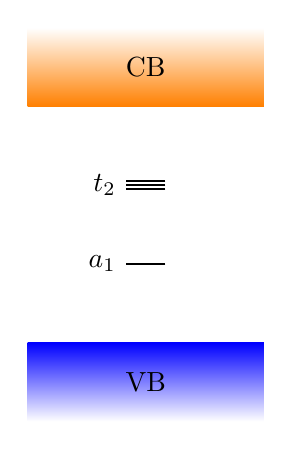
\begin{tikzpicture}

  \shade[top color=white,bottom color=orange] (0,-2.5) rectangle (3.0,-1.5) node[pos=.5] {CB};
  \shade[top color=blue,bottom color=white] (0.,-6.5) rectangle (3.0,-5.5) node[pos=.5] {VB};

  \draw[thick,-] (1.75,-4.5) -- (1.25,-4.5) node[anchor=east]{$a_1$};
  \draw[thick,-] (1.75,-3.5) -- (1.25,-3.5) node[anchor=east]{$t_2$};
  \draw[thick,-] (1.75,-3.55) -- (1.25,-3.55);
  \draw[thick,-] (1.75,-3.45) -- (1.25,-3.45);

  \atom[name=C, color=orange, scale=0.5]{
    gray/45/45/0,
    gray/315/315/0,
    gray/225/225/0,
    gray/135/135/0}
  \atom[name=C, color=orange, pos={(0.75,0.75)},scale=0.5]{
    gray/45/45/0,
    red/315/315/0,
    gray/225/225/0,
    gray/135/135/0}
  \atom[name=v, color=blue, pos={(1.5,0)},scale=0.5]{}
  \atom[name=C, color=orange, pos={(0.75,-0.75)},scale=0.5]{
    red/45/45/0,
    gray/315/315/0,
    gray/225/225/0,
    gray/135/135/0}
  \atom[name=C, color=orange, pos={(2.25,0.75)},scale=0.5]{
    gray/45/45/0,
    gray/315/315/0,
    red/225/225/0,
    gray/135/135/0}
  \atom[name=C, color=orange, pos={(2.25,-0.75)},scale=0.5]{
    gray/45/45/0,
    gray/315/315/0,
    gray/225/225/0,
    red/135/135/0}
  \atom[name=C, color=orange, pos={(3.0,0)},scale=0.5]{
      gray/45/45/0,
      gray/315/315/0,
      gray/225/225/0,
      gray/135/135/0}
\end{tikzpicture}
\subcaption{} \label{fig:defect diamond structure}
\end{subfigure}
\par\bigskip
\caption{A schematic representation of the electronic structure of a point defect in a tetrahedrally coordinated semiconductor, which is in this case diamond. Figure (a) shows the electronic states that correspond to the difference for an isolated atom and a lattice of atoms, as a superposition of $sp^3$ orbitals generates valence and conduction bands. In figure (b) a vacancy has been created by removing a carbon atom, and the four orbitals interact with each other resulting in two new states with $a_1$ and $t_2$ symmetry. The carbon atoms interact stronger with each other than the remaining four orbitals, which is why the two new states rests within the semiconductor's band gap. Figure adapted from ref. \cite{Gordon2013}.}
\label{fig: diamond electronic structure}
\end{figure}
